\documentclass{article}

\usepackage{vub}
%% PACKAGES

% Fancy chapters with toc
\usepackage{titlesec,titletoc}

\usepackage[style=alphabetic, maxnames=4]{biblatex}
\addbibresource{references.bib}

\usepackage{amsmath,amsfonts,amsthm,amssymb,mathtools}
\usepackage[shortlabels]{enumitem}
\usepackage{imakeidx}
\makeindex[intoc] % Add index to bibliography.
\usepackage[bookmarksdepth=2]{hyperref}
\usepackage{xcolor}
\hypersetup{
	colorlinks=true,
	linkcolor={red!50!black},
	citecolor={blue!50!black},
	urlcolor={blue!80!black}
}
\usepackage{cleveref}
\usepackage{tikz-cd}
\usepackage{aligned-overset}
\usepackage{tcolorbox}
\tcbuselibrary{breakable}
% \tcbuselibrary{theorems}
\tcbuselibrary{skins}
\usepackage{microtype}
\usepackage{nicematrix}
\NiceMatrixOptions{cell-space-limits = 5pt}

\renewcommand{\thechapter}{\Roman{chapter}}
\counterwithout{section}{chapter}
\counterwithout{figure}{chapter}
\counterwithout{table}{chapter}
\renewcommand*\thesection{\arabic{section}}

\titleformat{\chapter}[display]
{\bfseries\Large}
{\filleft
	\MakeUppercase{\chaptertitlename} \Huge\thechapter}
{3ex}
{\titlerule
	\vspace{2ex}%
	\filright}
[{%
			\vspace{2ex}%
			\titlerule
		}]

\titlecontents{chapter}
[0pt]
{\addvspace{1pc}}%
{\contentsmargin{0pt}%
	\bfseries
	\makebox[0pt][r]{\huge\thecontentslabel\enspace}%
	\large}
{% \addvspace{.2pc}%
	\contentsmargin{0pt}%
	\large}
{}
[\addvspace{.5pc}]

\newcommand{\chaptertoc}{%
	\dotfill
	\vspace*{1ex}
	\startcontents[chapters]
	\printcontents[chapters]{}{1}[2]{}
	\vspace*{1ex}
	\noindent\dotfill\\
	\vspace*{1pc}
}
% \usepackage{fancyhdr}
% \pagestyle{fancy}

\usetikzlibrary{positioning,quotes,calc,patterns}

%% Equation numbered by section
\numberwithin{equation}{section}

%% Theorem environments
\theoremstyle{plain}
\newtheorem{theorem}{Theorem}[section]
\newtheorem{lemma}[theorem]{Lemma}
\newtheorem{proposition}[theorem]{Proposition}
\newtheorem{corollary}[theorem]{Corollary}

\newtheorem{condition}{Condition}
\renewcommand*{\thecondition}{\Alph{condition}}
\crefname{condition}{condition}{conditions}

\newtheorem*{convention}{Convention}
\newtheorem*{theorem*}{Theorem}
\newtheorem*{lemma*}{Lemma}
\newtheorem*{prop*}{Proposition}
\newtheorem*{corollary*}{Corollary}

\theoremstyle{definition}
\newtheorem{definition}[theorem]{Definition}
% \newtheorem{example}[theorem]{Example}
\newtheorem{exercise}[theorem]{Exercise}
\newtheorem*{notation}{Notation}
\newtheorem*{definition*}{Definition}
\newtheorem*{example*}{Example}
\newtheorem*{exercise*}{Exercise}

\theoremstyle{remark}
\newtheorem{remark}[theorem]{Remark}
\newtheorem*{remark*}{Remark}

\tcolorboxenvironment{notation}{%
	blanker,breakable,left=5mm,
	before skip=10pt,after skip=10pt,
	borderline west={1mm}{0pt}{gray}}

\usepackage{thmtools}

\declaretheoremstyle[
  sibling=theorem,
	style=definition,
  spaceabove=1em plus 0.75em minus 0.25em,
  spacebelow=1em plus 0.75em minus 0.25em,
  qed={\itshape End of example.}
]{exmpstyle}

\declaretheorem[
  style=exmpstyle,
  title=Example,
  refname={example,examples},
  Refname={Example,Examples}
]{example}

%===========================================================%
%The code below customises theorem numbering
%===========================================================%

% \theoremstyle{plain}
% \newtheorem{innercustomgenericplain}{\customgenericname}
% \providecommand{\customgenericname}{}
% \newcommand{\newcustomtheoremplain}[2]{%
% 	\crefname{#2}{#2}{#2s}%
% 	\newenvironment{#1}[1]
% 	{%
% 		\renewcommand\customgenericname{#2}%
% 		\crefalias{innercustomgenericplain}{#2}%
% 		\renewcommand\theinnercustomgenericplain{##1}%
% 		\innercustomgenericplain
% 	}
% 	{\endinnercustomgenericplain}
% }

% \theoremstyle{definition}
% \newtheorem{innercustomgenericdefinition}{\customgenericname}
% \providecommand{\customgenericname}{}
% \newcommand{\newcustomtheoremdefinition}[2]{%
% 	\crefname{#2}{#2}{#2s}%
% 	\newenvironment{#1}[1]
% 	{%
% 		\renewcommand\customgenericname{#2}%
% 		\crefalias{innercustomgenericdefinition}{#2}%
% 		\renewcommand\theinnercustomgenericdefinition{##1}%
% 		\innercustomgenericdefinition
% 	}
% 	{\endinnercustomgenericdefinition}
% }

% \theoremstyle{remark}
% \newtheorem{innercustomgenericremark}{\customgenericname}
% \providecommand{\customgenericname}{}
% \newcommand{\newcustomtheoremremark}[2]{%
% 	\crefname{#2}{#2}{#2s}%
% 	\newenvironment{#1}[1]
% 	{%
% 		\renewcommand\customgenericname{#2}%
% 		\crefalias{innercustomgenericremark}{#2}%
% 		\renewcommand\theinnercustomgenericremark{##1}%
% 		\innercustomgenericremark
% 	}
% 	{\endinnercustomgenericremark}
% }

% \newcustomtheoremplain{customtheorem}{Theorem}
% \newcustomtheoremplain{customlemma}{Lemma}
% \newcustomtheoremplain{customprop}{Proposition}
% \newcustomtheoremplain{customcorollary}{Corollary}

% \newcustomtheoremdefinition{customdefinition}{Definition}
% \newcustomtheoremdefinition{customexample}{Example}
% \newcustomtheoremdefinition{customexercise}{Exercise}

% \newcustomtheoremremark{customremark}{Remark}

\input{definitions/macros}
\input{definitions/letterfonts}

\usetikzlibrary{shapes.geometric,calc, decorations.pathmorphing}

\newcommand{\ex}{\mathbf{ex}}
\newcommand{\frz}{\mathbf{frz}}
\newcommand{\bx}{\mathbf{x}}
\newcommand{\tbx}{\tilde{\bx}}
\newcommand{\tB}{\tilde{B}}
\DeclareMathOperator{\Fract}{Fract}

%%%%%%%%%%%%%
%% Fill in!%%
%%%%%%%%%%%%%
\title{Cluster Algebras}
\subtitle{Collection of notes on (quantum) cluster algebras}
\faculty{Sciences and Bio-Engineering Sciences}
\author{Wannes Malfait}
\date{Academic year 2023-2024}
\promotors{Kenny De Commer, Geoffrey Janssens}
% \pretitle{Dissertation for the grade of Master's in mathematics}

\begin{document}

\maketitle
\newpage
\tableofcontents
\newpage

\section{Classical cluster algebras}

Mostly use \cite{FominWilliams2021IntroductionCA_1-3} as reference together with
Geoffrey's notes.

\subsection{Combinatorial integer sequences}

In this section we will look at some integer sequences coming from number theory or
combinatorial data, and observe some interesting patterns. In the next section we will
see how these can all be viewed as special instances of a much more general framework.

Let us start with the simplest of the sequences.
\begin{definition}
	Let $a_n$ be the sequence defined through the recursion relation
	\begin{equation}
		\label{eq:somos_4}
		a_{n+4} = \frac{a_{n+3}a_{n+1}+ a_{n+2}^2}{a_n}
	\end{equation}
	with initial conditions $a_0 = a_1 = a_2 = a_3 = 1$. This sequence is known as the \emph{Somos-4}\index{Somos-4 sequence} sequence, named after its inventor, Michael Somos.
\end{definition}
Computing the first few terms of the sequence, we find:
\begin{align*}
	a_4    & = \frac{1 \cdot 1 + 1^2}{1} = 2                                           \\
	a_5    & = \frac{2 \cdot 1 + 1^2}{1} = 3                                           \\
	a_6    & = \frac{3 \cdot 1 + 2^2}{1} = 7                                           \\
	a_7    & = \frac{7 \cdot 2 + 3^2}{2} = 23                                          \\
	a_8    & = \frac{23 \cdot 3 + 7^2}{2} = \frac{118}{2} = 59                         \\
	a_9    & = \frac{59 \cdot 7 + 23^2}{3} = \frac{942}{3} = 314                       \\
	a_{10} & = \frac{314 \cdot 23 + 59^2}{7} = \frac{10703}{7} = 1529                  \\
	a_{11} & = \frac{1529 \cdot 59 + 314^2}{23} = \frac{188807}{23} = 8209             \\
	a_{12} & = \frac{8209 \cdot 314 + 1529^2}{59} = \frac{4915467}{59} = 83313         \\
	a_{13} & = \frac{83313 \cdot 1529 + 8209^2}{314} = \frac{194773258}{314} = 620297.
\end{align*}
From the definition of the sequence, there is no reason, a priori, to assume that all its elements would be integers. However, somewhat remarkably, the denominators seem to always cancel out perfectly. In the next section we will prove that all the terms in the sequence are indeed integers,
as a corollary of the \emph{Laurent phenomenon}\index{Laurent!phenomenon}.

The next family of integer sequences comes from \emph{$\SL_2(\bbZ)$-frieze
	patterns}\footnote{The name ``frieze pattern'' comes from architecture, where it refers
	to a horizontal strip, often found just below the roofline, which is decorated with
	patterns.}\index{Frieze pattern}. The idea of a frieze pattern is best explained
through an example (\cite{Coxeter1971FriezePatterns}). Take for example the following
pattern:
\begin{equation*}
	\dots\quad
	\begin{tikzcd}[
			sep = 0.2em, cramped,
		]
		&0&&0&&0&&0&&0&&0&&0&&0&&0&&0&&0\\
		1&&1&&1&&1&&1&&1&&1&&1&&1&&1&&1\\
		&1&&2&&2&&3&&1&&2&&4&&1&&2&&2&&3\\
		3&&1&&3&&5&&2&&1&&7&&3&&1&&3&&5\\
		&2&&1&&7&&3&&1&&3&&5&&2&&1&&7&&3\\
		4&&1&&2&&4&&1&&2&&2&&3&&1&&2&&4\\
		&1&&1&&1&&1&&1&&1&&1&&1&&1&&1&&1\\
		0&&0&&0&&0&&0&&0&&0&&0&&0&&0&&0
	\end{tikzcd}
	\quad
	\dots
\end{equation*}
The defining property is that the $2 \times 2$ diamonds
\begin{equation*}
	\begin{matrix}
		  & b &   \\
		a &   & d \\
		  & c &
	\end{matrix}
\end{equation*}
formed by adjacent elements, can be seen as an element of $\SL_2 (\bbZ)$, i.e., $ad - bc = 1$. Other than the bounding rows of ones and zeros, there is no additional requirement. In what follows we will omit the irrelevant row of zeros. One could ask if it is always possible to construct such a pattern for any number of rows. If so, one might be interested in knowing how many such patterns there are. Furthermore, one might notice that the pattern is periodic, repeating every 7 columns. In fact, the pattern even has ``half-periodicity'' where the marked triangle undergoes a translation and reflection.
\begin{equation*}
	\dots\quad
	\begin{tikzcd}[
			sep = 0.2em, cramped,
			execute at end picture = {
					\draw[blue, dashed, rounded corners]
					($(\tikzcdmatrixname-1-1.north west) + (-0.3, 0.05)$) -- ($(\tikzcdmatrixname-1-11.north east)+ (0.3, 0.05)$)--($(\tikzcdmatrixname-6-6.south) + (0,-0.05)$) -- cycle;
					\draw[red, dashed, rounded corners]
					($(\tikzcdmatrixname-6-8.south west) + (-0.3, -0.05)$) -- ($(\tikzcdmatrixname-6-18.south east)+ (0.3, -0.05)$)--($(\tikzcdmatrixname-1-13.north) + (0,0.05)$) -- cycle;
				}
		]
		1&&1&&1&&1&&1&&1&&1&&1&&1&&1&&1\\
		&1&&2&&2&&3&&1&&2&&4&&1&&2&&2&&3\\
		3&&1&&3&&5&&2&&1&&7&&3&&1&&3&&5\\
		&2&&1&&7&&3&&1&&3&&5&&2&&1&&7&&3\\
		4&&1&&2&&4&&1&&2&&2&&3&&1&&2&&4\\
		&1&&1&&1&&1&&1&&1&&1&&1&&1&&1&&1\\
	\end{tikzcd}
	\quad
	\dots
\end{equation*}

To make such a pattern, we start with the observation that the rest of the pattern is
completely determined by a lattice path from top to bottom. Indeed, using the
$\SL_2(\bbZ)$ rule, one can fill in the rest of the pattern. For example, say we
started with the following partially filled in pattern:
\begin{equation*}
	\dots\quad
	\begin{tikzcd}[
			sep = 0.2em, cramped,
		]
		1&&1&&1&&1&&1&&1&&1\\
		&a\\
		b\\
		&1&&1&&1&&1&&1&&1\\
	\end{tikzcd}
	\quad
	\dots
\end{equation*}
then we could fill out the rest as follows
\begin{equation*}
	\dots\quad
	\begin{tikzcd}[
			sep = 0.2em, cramped,
		]
		1&&1&&1&&1&&1&&1&&1\\
		&a&& \frac{1+a+b}{ab} && b && \frac{1+a}{b} && \frac{1+b}{a} && a\\
		b&& \frac{1+a}{b} &&  \frac{1+b}{a} && a && \frac{1+a+b}{ab} && b\\
		&1&&1&&1&&1&&1&&1\\
	\end{tikzcd}
	\quad
	\dots
\end{equation*}
Since all the denominators are monomials in $a$ and $b$, it follows that when $a = b = 1$, all the
elements will be integers, as required.

It seems that we somehow got lucky in this case. There is again, a priori, no reason to
assume that for any number of rows, we will always be able to choose the initial
integers such that all the fractions simplify. The fact that this is possible, follows
again from the ``Laurent phenomenon''\index{Laurent!phenomenon}, on which we can now
shed a bit more light. Let $a_1, a_2, \dots, a_n$ be the initial integers chosen on the
lattice path. Then, in this context, the Laurent phenomenon states that all the other
elements of the frieze pattern can be written as Laurent
polynomials\index{Laurent!polynomial} in $a_1 , \dots, a_n$ with coefficients in
$\bbZ$, i.e., as an element of $\bbZ [a_1 ^\pm, \dots, a_n^\pm]$. So, any lattice path
from top to bottom consisting of only ones, will yield a frieze pattern. This already
proves the existence of such frieze patterns for any number of rows. We will return to
the other questions in the next section.

Let us now look at a final example, coming from triangulations of $n$-gons. We first
recall the following theorem from Euclidean geometry.
\begin{theorem}[Ptolomy's Theorem]
	Let $A,B,C,D$ be distinct points on a circle, in cyclic order (\cref{fig:ptolomy}).
	These determine vertices of a quadrilateral, where the side, and diagonal lengths
	satisfy the following rule:
	\begin{equation*}
		|AC| \cdot |BD| = |AB|\cdot |CD| + |AD| \cdot |BC|.
	\end{equation*}
\end{theorem}

\begin{figure}
	\centering

	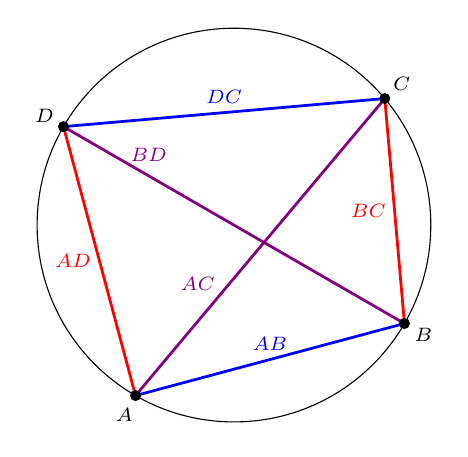
\begin{tikzpicture}
		\coordinate (center) at (0,0);
		\def\radius{2.5cm}
		\draw (center) circle[radius=\radius];

		% points on the circle
		\path (center) ++(-120:\radius) coordinate (A);
		\path (center) ++(-30:\radius) coordinate (B);
		\path (center) ++(40:\radius) coordinate (C);
		\path (center) ++(150:\radius) coordinate (D);

		\begin{scriptsize}
			% Chords
			\draw[color=red, line width=1pt] (A) -- node[left] {$AD$} (D);
			\draw[color=red, line width=1pt] (B) -- node[left] {$BC$} (C);
			\draw[color=blue, line width=1pt] (A) -- node[above] {$AB$} (B);
			\draw[color=blue, line width=1pt] (D) -- node[above] {$DC$} (C);
			\draw[color=violet, line width=1pt] (A) -- node[above=8pt, near start] {$AC$} (C);
			\draw[color=violet, line width=1pt] (D) -- node[above=2pt, near start] {$BD$} (B);

			% Draw the points over the chords
			\fill[black] (A) circle[radius=2pt] ++(-120:1em) node {$A$};
			\fill[black] (B) circle[radius=2pt] ++(-30:1em) node {$B$};
			\fill[black] (C) circle[radius=2pt] ++(40:1em) node {$C$};
			\fill[black] (D) circle[radius=2pt] ++(150:1em) node {$D$};

		\end{scriptsize}
	\end{tikzpicture}
	\caption{Ptolomy's theorem:
	${\color{violet} |AC| \cdot |BD|}
		= {\color{red} |AD|\cdot |BC|} + {\color{blue} |AB| \cdot |CD|}$.}
	\label{fig:ptolomy}
\end{figure}

This rule allows to compute the length of one of the diagonals in terms of the other,
given the side lengths. We will now apply this to triangulations of polygons.

Let $1, 2, \dots, n$ denote $n$ points on a circle, arranged in cyclic order. By
connecting these points through sides $P_{i, i+1}$, where the indices are taken modulo
$n$, we obtain a polygon with $n$-sides. A triangulation\index{Triangulations!of
	polygons}, $T$, is a choice of $(n-3)$ non-crossing diagonals. This results in a
partitioning of the polygon in $n-2$ triangles. We will see triangulations in much more
detail in a later section, and will therefore keep things brief here. For now, it is
enough to understand things visually (cf. \cref{fig:triangulations}).

\begin{figure}
	\centering

	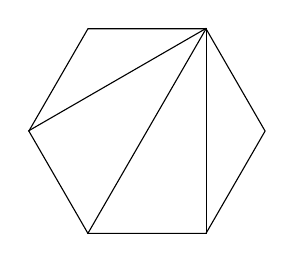
\begin{tikzpicture}
		\node[name=h, shape=regular polygon, draw, regular polygon sides = 6, minimum size = 3cm]{};
		\draw[] (h.corner 1) -- (h.corner 3);
		\draw[] (h.corner 1) -- (h.corner 4);
		\draw[] (h.corner 1) -- (h.corner 5);
	\end{tikzpicture}
	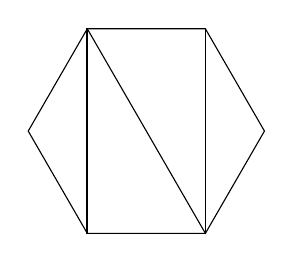
\begin{tikzpicture}
		\node[name=h, shape=regular polygon, draw, regular polygon sides = 6, minimum size = 3cm]{};
		\draw[] (h.corner 2) -- (h.corner 5);
		\draw[] (h.corner 2) -- (h.corner 4);
		\draw[] (h.corner 1) -- (h.corner 5);
	\end{tikzpicture}
	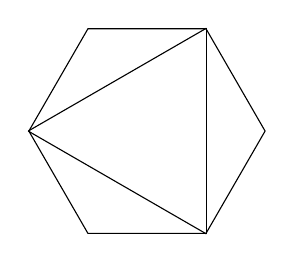
\begin{tikzpicture}
		\node[name=h, shape=regular polygon, draw, regular polygon sides = 6, minimum size = 3cm]{};
		\draw[] (h.corner 1) -- (h.corner 3);
		\draw[] (h.corner 3) -- (h.corner 5);
		\draw[] (h.corner 1) -- (h.corner 5);
	\end{tikzpicture}

	\caption{Some triangulations of a hexagon.}
	\label{fig:triangulations}
\end{figure}

Starting from a triangulation, $T$, we obtain a new triangulation, $T'$, by
``flipping'' a diagonal. Any diagonal in a triangulation lies on precisely 2 triangles.
These two triangles form a quadrilateral. To flip the diagonal, you replace it with the
other diagonal of that quadrilateral. Again, this is most easily seen visually:
\begin{equation*}
	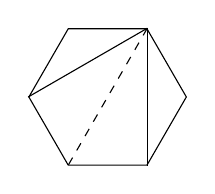
\begin{tikzpicture}[baseline]
		\node[name=h, shape=regular polygon, draw, regular polygon sides = 6, minimum size = 2cm]{};
		\draw[] (h.corner 1) -- (h.corner 3);
		\draw[dashed] (h.corner 1) -- (h.corner 4);
		\draw[] (h.corner 1) -- (h.corner 5);
	\end{tikzpicture}
	\quad \leadsto \quad
	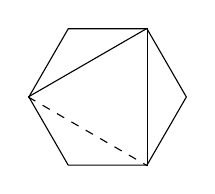
\begin{tikzpicture}[baseline]
		\node[name=h, shape=regular polygon, draw, regular polygon sides = 6, minimum size = 2cm]{};
		\draw[] (h.corner 1) -- (h.corner 3);
		\draw[dashed] (h.corner 3) -- (h.corner 5);
		\draw[] (h.corner 1) -- (h.corner 5);
	\end{tikzpicture}
\end{equation*}
%
Now, using Ptolomy's theorem, the length of the new diagonal can be computed given that
we knew the lengths of all the edges in the previous triangulation. We now ignore
Euclidean geometry, and just use Ptolomy's theorem as a recurrence relation to
construct a collection of numbers as follows: Pick a triangulation and set all the edge
lengths equal to one. Then at each step, choose a diagonal in the triangulation and
flip it. Compute its edge length using Ptolomy's theorem. This is the next number in
the collection. For example, we could obtain a sequence starting like this (we omit the
ones on the sides):
\begin{equation*}
	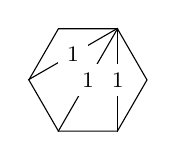
\begin{tikzpicture}[baseline]
		\node[name=h, shape=regular polygon, draw, regular polygon sides = 6, minimum size = 1.5cm]{};
		\draw[] (h.corner 1) -- node[fill=white, font=\footnotesize] {1} (h.corner 3);
		\draw[] (h.corner 1) -- node[fill=white, font=\footnotesize] {1} (h.corner 4);
		\draw[] (h.corner 1) -- node[fill=white, font=\footnotesize] {1} (h.corner 5);
	\end{tikzpicture}
	\leadsto
	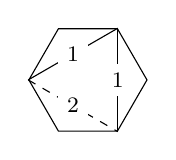
\begin{tikzpicture}[baseline]
		\node[name=h, shape=regular polygon, draw, regular polygon sides = 6, minimum size = 1.5cm]{};
		\draw[] (h.corner 1) -- node[fill=white, font=\footnotesize] {1} (h.corner 3);
		\draw[dashed] (h.corner 3) -- node[fill=white, font=\footnotesize] {2} (h.corner 5);
		\draw[] (h.corner 1) -- node[fill=white, font=\footnotesize] {1} (h.corner 5);
	\end{tikzpicture}
	\leadsto
	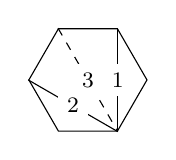
\begin{tikzpicture}[baseline]
		\node[name=h, shape=regular polygon, draw, regular polygon sides = 6, minimum size = 1.5cm]{};
		\draw[dashed] (h.corner 2) -- node[fill=white, font=\footnotesize] {3} (h.corner 5);
		\draw[] (h.corner 3) -- node[fill=white, font=\footnotesize] {2} (h.corner 5);
		\draw[] (h.corner 1) -- node[fill=white, font=\footnotesize] {1} (h.corner 5);
	\end{tikzpicture}
	\leadsto
	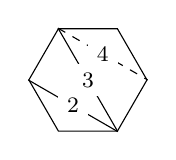
\begin{tikzpicture}[baseline]
		\node[name=h, shape=regular polygon, draw, regular polygon sides = 6, minimum size = 1.5cm]{};
		\draw[] (h.corner 2) -- node[fill=white, font=\footnotesize] {3} (h.corner 5);
		\draw[] (h.corner 3) -- node[fill=white, font=\footnotesize] {2} (h.corner 5);
		\draw[dashed] (h.corner 2) -- node[fill=white, font=\footnotesize] {4} (h.corner 6);
	\end{tikzpicture}
	\leadsto
	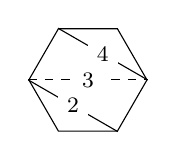
\begin{tikzpicture}[baseline]
		\node[name=h, shape=regular polygon, draw, regular polygon sides = 6, minimum size = 1.5cm]{};
		\draw[dashed] (h.corner 3) -- node[fill=white, font=\footnotesize] {3} (h.corner 6);
		\draw[] (h.corner 3) -- node[fill=white, font=\footnotesize] {2} (h.corner 5);
		\draw[] (h.corner 2) -- node[fill=white, font=\footnotesize] {4} (h.corner 6);
	\end{tikzpicture}
	\leadsto
	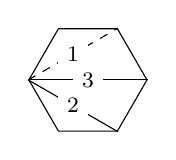
\begin{tikzpicture}[baseline]
		\node[name=h, shape=regular polygon, draw, regular polygon sides = 6, minimum size = 1.5cm]{};
		\draw[] (h.corner 3) -- node[fill=white, font=\footnotesize] {3} (h.corner 6);
		\draw[] (h.corner 3) -- node[fill=white, font=\footnotesize] {2} (h.corner 5);
		\draw[dashed] (h.corner 3) -- node[fill=white, font=\footnotesize] {1} (h.corner 1);
	\end{tikzpicture}
	\leadsto \cdots
\end{equation*}
%
Once again, we observe that we only obtain integers. Furthermore, there seems to be a
limit to which integers we can obtain this way. This hints at a hidden periodicity. The
Laurent phenomenon offers an explanation for why we only obtain integers: the lengths
of the diagonals are Laurent polynomials in the originally chosen lengths.

There are many more examples like the three that we just gave. One can look at wiring
diagrams, generalized Somos sequences, Markov Triples, knight recurrence, the
Gale-Robinson sequence, etc. As the focus of this thesis is not on number theory, we
refrain from delving deeper into this interesting world. We refer interested readers to
\cite[Chapter 3.4]{FominWilliams2021IntroductionCA_1-3} and
\cite{FominZelevinsky2002Laurent}.

\subsection{Quivers and mutations}

As observed in the previous section, the examples share some common features. The most
prominent of these was the Laurent phenomenon. There are some more subtle similarities,
which will become clear in this section. The main role will be played by quivers, and
their mutations.

\begin{definition}[Quivers]
	A \emph{quiver}\index{Quiver} is a finite directed (multi)-graph with no 1-cycles (vertex connected to itself) or 2-cycles (two vertices connected by a pair of opposite arrows) (cf. \cref{fig:triangulations}).
\end{definition}

\begin{figure}
	\centering
	\begin{equation*}
		\begin{tikzcd}
			&\bullet \arrow[loop] \arrow[r] &\bullet \\
			\bullet \rar & \bullet \arrow[r, bend left] & \bullet \arrow[l, bend left]
		\end{tikzcd}
		\hspace{2cm}
		\begin{tikzcd}[row sep=small]
			&&& \bullet \\
			\bullet \ar[rrrd, bend right]\rar &\bullet  \rar[leftarrow] &\bullet \ar[ru, shift left] \ar[ru, shift right] \ar[rd] \\
			&&& \bullet\\
			\\
			\bullet \ar[rr] && \bullet \ar[ld]\\
			& \bullet \ar[lu]
		\end{tikzcd}
	\end{equation*}
	\caption{The graphs on the left are not quivers, the graphs on the right are.}
	\label{fig:quivers}
\end{figure}

We will now fix some notation for what follows. Write $[a,b] = \{a, a + 1, \dots, b\}$
for integers $a,b \in \bbZ$, where $[a,b] = \emptyset$ if $a > b$. Now, fix an integer
$N$, and a subset $\ex subset.eq [1, N]$ of size $n$. The elements of $\ex$ will be
called \emph{exchangeable}\index{Exchangeable}, while the elements of $\frz = [1, N]
	\setminus \ex$ will be called \emph{frozen}\index{Frozen}. Finally, let $\mcF = \bbQ
	(X_1, \dots, X_N)$ be the field of rational functions over $\bbQ$, in $N$ variables.

\begin{definition}
	We call a pair $(Q, \tbx)$ a \emph{seed}\index{Seed} if
	\begin{enumerate}
		\item $Q$ is a quiver with vertices $Q_0 = [1, N]$.
		\item $\tbx = \{x_1, \dots, x_N\}$ is a \emph{free generating set} of $\mcF$. That is, $\tbx$ is a set of $N$ algebraically independent elements that generate $\mcF$.
	\end{enumerate}
	The set $\bx = \{x_i \mid i \in \ex\} \subseteq \tbx$ will be referred to as the \emph{cluster}\index{Cluster}. The elements of $\bx$ will be called \emph{cluster variables}\index{Cluster!variables}.
\end{definition}

Although not strictly necessary, we will assume that the quiver $Q$ contains no arrows
between the frozen vertices, i.e., the vertices in $Q_0 \cap \frz$. Arrows between
exchangeable and frozen vertices are allowed. When drawing a quiver, the frozen
vertices will be drawn with a box, while the exchangeable vertices will just be drawn
normally.

Given a seed, we can convert it to another seed through a \emph{seed
	mutation}\index{Seed!mutation}.
\begin{definition}
	Let $k \in \ex$ be an exchangeable vertex of the quiver $Q$.
	We define the \emph{mutation in direction $k$} of the seed
	$(Q, \tbx)$ to be the seed $\mu_k(Q, \tbx) = (Q', \tbx')$, where
	\begin{enumerate}
		\item $Q'_0 = Q_0$.
		\item For every pair of vertices $i,j$ with $s$ arrows $i \to k$ and $t$ arrows $k \to j$ we
		      ``collapse'' these arrows into $s\cdot t$ arrows $i \to j$, cancelling pairwise with
		      any arrows $j \to i$.
		      \begin{equation*}
			      \begin{tikzcd}[column sep=small]
				      i \ar[rr, "r"] \ar[rd, "s"] && j \\
				      & k \ar[ur, "t"]
			      \end{tikzcd}
			      \quad \begin{tikzcd}
				      \; \rar[rightsquigarrow, "\mu_k"]& \;
			      \end{tikzcd}\quad
			      \begin{tikzcd}[column sep=small]
				      i \ar[rr, "r + st"] \ar[rd,leftarrow, "s"] && j \\
				      & k \ar[ur, leftarrow, "t"]
			      \end{tikzcd}
		      \end{equation*}
		      Here we take $r$ to be negative, if the arrows actually point the other way.
		      If $i,j$ are both frozen, then we ignore this step.
		\item All arrows in $Q$ incident to $k$ get their orientation flipped.
		\item $\tbx' = \{x_1', \dots, x_n'\}$, where $x_i' = x_i$ for $i \neq k$, and $x'_k$
		      is given by the \emph{exchange relation}\index{Exchange relation}
		      \begin{equation*}
			      x'_k = \frac{1}{x_k} \left(\prod_{i \to k} x_i + \prod_{k \to j} x_j\right),
		      \end{equation*}
		      where we take the product equal to 1 if $\{i \to k\} = \emptyset$ or $\{k \to j\} = \emptyset$.
	\end{enumerate}
\end{definition}

Before we give some examples, we prove a small lemma, which will also be useful for the
examples.
\begin{lemma}\label{lem:mutation_involution}
	Seed mutation at a fixed vertex is an involution, i.e., $\mu_k \circ \mu_k = id$.
\end{lemma}

\begin{proof}
	We first show that the quiver remains unchanged. For arrows incident to $k$, the
	mutation reverses the orientation. So, applying it twice yields the same orientation.
	Now, the only other part of the quiver that changes is at pairs of vertices $i,j$ with
	$s$ arrows $i \to k$ and $t$ arrows $k \to j$. Applying a single mutation introduces
	$s\cdot t$ new arrows $i \to j$. When applying the mutation the second time, we now
	have $s$ arrows $k \to i$ and $t$ arrows $j \to k$, due to the orientation flip of the
	arrows incident to $k$. Consequently, the mutation introduces $s \cdot t$ arrows $j \to
		i$ which cancel out exactly the arrows from the first mutation.

	To see that the cluster variables remain unchanged is a simple calculation:
	\begin{align*}
		x_k''
		 & = \frac{1}{x_k'}\left(\prod_{k \to i}x_i' + \prod_{j \to k} x_j'\right)                                                \\
		 & = x_k \left(\prod_{i \to k} x_i + \prod_{k \to j}x_j\right)^{-1} \left(\prod_{k \to i}x_i + \prod_{j \to k} x_j\right) \\
		 & = x_k,
	\end{align*}
	where we use that the exchange rule is unchanged by an orientation flip of all the arrows.
\end{proof}

We begin with an example to illustrate the mutation of the quiver.
\begin{example}
	We mutate the given quiver at vertex 2:
	\begin{equation*}
		\begin{tikzcd}
			& 4 \dlar \rar & 6 \dar \\
			1 \rar & 2 \uar \rar \dar[shift left] \dar [shift right] & 5 \\
			& 3 \ular
		\end{tikzcd}
		\begin{tikzcd}
			\; \rar[rightsquigarrow, "\mu_2"] &\;
		\end{tikzcd}
		\begin{tikzcd}
			& 4 \rar \dar & 6 \dar \\
			1  \drar \ar[rr,controls = {+(1, -2) and +(-1, -2)}] & 2 \lar & 5 \lar \\
			& 3 \uar[shift right] \uar[shift left]
		\end{tikzcd}
	\end{equation*}
	%
	The arrow $1 \to 2$ combined with the arrow $2 \to 4$ introduces one new arrow $1 \to
		4$ which cancels out the existing arrow $4 \to 1$. The arrow $1 \to 2$ combines with
	the 2 arrows $2 \to 3$ to create 2 new arrows $1 \to 3$,one of which cancels out with
	the existing arrow $3 \to 1$. Finally, the arrow $1 \to 2$ combined with the arrow $2
		\to 5$ yields an arrow $1 \to 5$. The arrows incident to the vertex 6 remain unchanged.
\end{example}

Let us now look at some examples, where we also keep track of the cluster variables.
\begin{example}
	The simplest example is the quiver consisting of a single vertex:
	\begin{equation*}
		Q = \begin{tikzcd}
			\bullet
		\end{tikzcd},
		\quad \bx = \{x\}.
	\end{equation*}
	%
	Mutating at the only vertex gives
	\begin{equation*}
		Q = \begin{tikzcd}
			\bullet
		\end{tikzcd},
		\quad \bx = \left\{\frac{x}{2}\right\}.
	\end{equation*}
	%
	If we mutate again, we end up with the original seed, as a consequence of
	\cref{lem:mutation_involution}. It is of course also straightforward to verify
	directly.
\end{example}
\begin{example}
	The next simplest example is the $A_2$ quiver:
	\begin{equation*}
		Q = \begin{tikzcd}
			1 \rar &2
		\end{tikzcd},
		\quad \bx = \left\{x_1, x_2\right\}.
	\end{equation*}
	%
	If we apply a mutation at the first vertex, we obtain:
	\begin{equation*}
		\mu_1(Q) = \begin{tikzcd}
			1 & \lar 2
		\end{tikzcd},
		\quad \mu_1(\bx) = \left\{\frac{1+x_2}{x_1}, x_2\right\}.
	\end{equation*}
	%
	We already know that mutating at the first vertex again will yield the same seed, so
	the only interesting thing to do is to see what happens after mutating at index 2:
	\begin{equation*}
		\mu_2(\mu_1(Q)) = \begin{tikzcd}
			1 \rar & 2
		\end{tikzcd},
		\quad  \mu_2(\mu_1(\bx)) = \left\{\frac{1+x_2}{x_1}, \frac{x_1 + x_2 + 1}{x_2}\right\}.
	\end{equation*}
	%
	Although we are back at the original quiver, the cluster variables are completely
	different. We now mutate again at the first vertex. We will use the notation
	$\mu_{k_1k_2\cdots k_l}$ as a shorthand for $\mu_{k_l} \circ \cdots \circ \mu_{k_2}
		\circ \mu_{k_1}$.
	\begin{equation*}
		\mu_{121}(Q) = \begin{tikzcd}
			1 &\lar 2
		\end{tikzcd},
		\quad  \mu_{121}(\bx) = \left\{\frac{x_1(x_1 x_2 + x_1 + x_2 + 1)}{x_1x_2(1+x_2)}, \frac{x_1 + x_2 + 1}{x_2}\right\}.
	\end{equation*}
	%
	The expression for the first cluster variable looks complicated, but can be
	dramatically simplified to $\frac{x_1 + 1}{x_2}$. We continue mutating:
	\begin{equation*}
		\mu_{1212}(Q) = \begin{tikzcd}
			1 \rar& 2
		\end{tikzcd},
		\quad  \mu_{1212}(\bx) = \left\{\frac{x_1 + 1}{x_2}, x_1\right\}.
	\end{equation*}
	%
	Once again, some simplification has taken place. We mutate a final time at the first
	vertex.
	\begin{equation*}
		\mu_{12121}(Q) = \begin{tikzcd}
			1 &\lar 2
		\end{tikzcd},
		\quad  \mu_{12121}(\bx) = \left\{x_2, x_1\right\}.
	\end{equation*}

	We have our original seed, except that the arrow in the quiver has been reversed, and
	that $x_1$ and $x_2$ have swapped places. In other words, after 5 mutations, the roles
	of 1 and 2 have swapped. It follows that another 5 swaps will give back the original
	seed. If one takes a close look at the obtained cluster variables, then we see that
	these correspond exactly to those that we found when trying to construct a frieze
	pattern with 2 rows. This is no coincidence, and we will come back to this later.
\end{example}
\begin{example}
	In this example, we look at the Markov quiver:
	\begin{equation*}
		\begin{tikzcd}[column sep= small]
			& 1 \ar[ld, shift left] \ar[ld, shift right]\\
			2 \ar[rr, shift left] \ar[rr, shift right] && 3 \ar[lu, shift left] \ar[lu, shift right]
		\end{tikzcd},
	\end{equation*}
	%
	which possesses the special property that it remains invariant under mutations at any
	vertex. Let us see what happens to the cluster variables as we mutate in a cyclic order
	of the vertices:
	\begin{align*}
		\bx            & = \{x, y, z\}                                                                                                                                                                               \\
		\mu_1(\bx)     & = \left\{\frac{y^2 + z^2}{x}, y, z\right\}                                                                                                                                                  \\
		\mu_{12}(\bx)  & = \left\{\frac{y^2 + z^2}{x}, \frac{y^4 + 2 z^2y^2 +z^4 + z^2x^2 }{x^2y}, z\right\}                                                                                                         \\
		\mu_{123}(\bx) & = \left\{\frac{y^2 + z^2}{x}, \frac{y^4 + 2 z^2y^2 +z^4 + z^2x^2 }{x^2y},\right.                                                                                                            \\
		               & \left. \frac{x^{4} z^{4} + x^{2} y^{6} + 4 x^{2} y^{4} z^{2} + 5 x^{2} y^{2} z^{4} + 2 x^{2} z^{6} + y^{8} + 4 y^{6} z^{2} + 6 y^{4} z^{4} + 4 y^{2} z^{6} + z^{8}}{x^{4} y^{2} z} \right\}
	\end{align*}
	%
	Mutating again at the first vertex gives the new cluster variable
	\begin{align*}
		 & \frac{x^{8} z^{6} + 4 x^{6} y^{4} z^{4} + 8 x^{6} y^{2} z^{6} + 4 x^{6} z^{8} + x^{4} y^{10} + 8 x^{4} y^{8} z^{2} + 24 x^{4} y^{6} z^{4} + 34 x^{4} y^{4} z^{6} + 23 x^{4} y^{2} z^{8}}{x^7y^4z^2} \\&+ \frac{6 x^{4} z^{10} + 2 x^{2} y^{12} + 14 x^{2} y^{10} z^{2} + 40 x^{2} y^{8} z^{4} + 60 x^{2} y^{6} z^{6} + 50 x^{2} y^{4} z^{8} + 22 x^{2} y^{2} z^{10} + 4 x^{2} z^{12}}{x^7 y^4 z^2}\\ &+ \frac{y^{14} + 7 y^{12} z^{2} + 21 y^{10} z^{4} + 35 y^{8} z^{6} + 35 y^{6} z^{8} + 21 y^{4} z^{10} + 7 y^{2} z^{12} + z^{14}}{x^{7} y^{4} z^{2}}.
	\end{align*}
	%
	Because the author doesn't want to spend too much time fiddling with alignment points
	to get long fractions to fit on a page, we will stop here. Mutating at vertex 2 would
	yield another fraction with 65 terms (with positive integer coefficients) in the
	numerator, and the expression $x^{12}y^7z^4$ in the denominator.
\end{example}

\begin{example}
	As a last example, we look at the $A_3$ quiver
	\begin{equation*}
		Q =
		\begin{tikzcd}
			1 \rar[] & 2 \rar[] &3
		\end{tikzcd},
		\quad \bx = \left\{x_1, x_2, x_3\right\}.
	\end{equation*}
	Mutation in direction 2 gives
	\begin{equation*}
		\mu_2(Q) =
		\begin{tikzcd}
			1 \rar[leftarrow] \ar[rr, bend right] & 2 \rar[leftarrow]& 3
		\end{tikzcd},
		\quad \mu_2(\bx) = \left\{x_1, \frac{x_1 + x_3}{x_2}, x_3\right\}.
	\end{equation*}
	If we instead apply a mutation in direction 1, we find
	\begin{equation*}
		\mu_1(Q) =
		\begin{tikzcd}
			1 \rar[leftarrow] & 2 \rar[]& 3
		\end{tikzcd},
		\quad \mu_1(\bx) = \left\{\frac{x_2 + 1}{x_1}, x_2, x_3\right\}.
	\end{equation*}
	Finally, a mutation in direction 3 would give
	\begin{equation*}
		\mu_3(Q) =
		\begin{tikzcd}
			1 \rar[] & 2 \rar[leftarrow]& 3
		\end{tikzcd},
		\quad \mu_3(\bx) = \left\{x_1, x_2, \frac{x_2 + 1}{x_3}\right\}.
	\end{equation*}
	Mutating in direction 1 on $\mu_2(Q)$ gives
	\begin{equation*}
		\mu_{21}(Q) =
		\begin{tikzcd}
			1 \rar[] \ar[rr,leftarrow, bend right] & 2 & 3
		\end{tikzcd},
		\quad \mu_{21}(\bx) = \left\{\frac{x_1 + x_3 + x_2x_3}{x_1x_2}, \frac{x_1 + x_3}{x_2}, x_3\right\}.
	\end{equation*}
	If we now mutate in direction 3, we obtain
	\begin{equation*}
		\mu_{213}(Q) =
		\begin{tikzcd}
			1 \rar[] \ar[rr, bend right] & 2 & 3
		\end{tikzcd},
		\quad \mu_{213}(\bx) = \left\{\frac{x_1 + x_3 + x_2x_3}{x_1x_2}, \frac{x_1 + x_3}{x_2}, \frac{x_1 x_2 + x_1 + x_3 + x_2 x_3}{x_1x_2x_3}\right\}.
	\end{equation*}
	It seems that the expressions keep getting messier and messier. We mutate again in direction 2:
	\begin{equation*}
		\mu_{2132}(Q) =
		\begin{tikzcd}
			1 \rar[leftarrow] \ar[rr, bend right] & 2 & 3
		\end{tikzcd},
	\end{equation*}
	\begin{equation*}
		\mu_{2132}(\bx)= \left\{\frac{x_1 + x_3 + x_2x_3}{x_1x_2}, \frac{x_2 + 1}{x_1}, \frac{x_1 x_2 + x_1 + x_3 + x_2 x_3}{x_1x_2x_3}\right\}.
	\end{equation*}
	Somehow, some miraculous cancelation happened.
	Note that the expression $\frac{x_2 + 1}{x_2}$ already appeared previously.
	If we instead mutate in direction 1, we get
	\begin{equation*}
		\mu_{2131}(Q) =
		\begin{tikzcd}
			1 \rar[leftarrow] \ar[rr,leftarrow, bend right] & 2 & 3
		\end{tikzcd},
	\end{equation*}
	\begin{equation*}
		\mu_{2131}(\bx) = \left\{\frac{x_1 + x_3 + x_1x_2}{x_2x_3}, \frac{x_1 + x_3}{x_2}, \frac{x_1 x_2 + x_1 + x_3 + x_2 x_3}{x_1x_2x_3}\right\}.
	\end{equation*}
	This still introduces a new expression.
	Interestingly, these are all the possible expressions we can obtain!
	If we now mutate in, say, direction 3, we would get as cluster
	\begin{equation*}
		\mu_{21313} = \left\{\frac{x_1 + x_3 + x_1x_2}{x_2x_3}, \frac{x_1 + x_3}{x_2}, x_1 \right\}.
	\end{equation*}
	This is again a dramatic cancelation. One can check manually
	that no mutations introduce new cluster variables.
\end{example}

From these examples we can observe a few things:
\begin{enumerate}
	\item Even though a sequence of mutations might result in the same quiver, the corresponding
	      cluster variables might be different.
	\item For some quivers, the number of obtainable cluster variables is finite.
	\item Independent of the quiver, all the cluster variables are Laurent polynomials in the
	      original cluster variables.
	\item The Laurent polynomials have coefficients in the positive integers.
\end{enumerate}

We will now explain each of the observations in more detail.

Motivate as way to generalize phenomenon from previous subsection. What is a quiver and
seed, frozen and exchangeable variables. Mutation. The Laurent phenomenon and total
positivity.

Write out example of $A_3$ and non-finite type. Classification of cluster-finite
quivers. Another remark is that the total number of cluster variables we obtained was
$9 = 3 + 6$. It is no coincidence that $A_3$ is a Dynkin diagram of rank 3, and that
the corresponding root system has $6$ positive roots. The positive roots correspond to
the denominators that appear in the cluster variables.

\subsection{The Grassmannian}
Definition of Grassmannian. Plucker coordinates, algebra relations. Special case of
$k=2$. Correspondence with triangulations.
\subsection{Triangulations of surfaces}
Explain how to generalize to marked surfaces with punctures.
\section{Quantum cluster algebras}

\subsection{Quantum tori}

Some of the basic background needed on quantum tori, and rational actions.

\subsection{Quantum cluster algebras}

Toric frames, quantum seeds and mutations. Quantum Laurent phenomenon.

\subsection{Quantum Grassmannians}
???

\subsection{CGL extensions}

What is CGL extension. Main theorem from \cite{GoodearlYakimov2017QCA}. Key parts of
proof needed to get there. Have an example along the way.

\section{Some definitions}

We start with the non-quantized version of cluster algebras, introduced in
\cite{FominZelevinsky2002CAF}. We won't take the most general definition, since that
doesn't carry over as nicely to the quantized version.

\subsection{Notation}

Some of the notation that we will use throughout this paper. Let $[a,b] = \{a, a+1,
	\dots, b\}$ for integers $a,b \in \bbZ$, where $[a,b] = \emptyset$ if $a > b$. Fix an
integer $N$, and a subset $\ex \subseteq [1, N]$ of size $n$. The elements of $\ex$
will be called the \emph{exchangeable} indices. Let $\mcF = \bbQ(Y_1, \dots, Y_N)$, be
the field of rational functions over $\bbQ$. Boldface letters will be used to denote
vectors, matrices, or clusters.

\subsection{Classical cluster algebras}

Before giving the definition of a cluster algebra, we need to define what seeds and
seed mutations are.
\begin{definition}[\cite{BerensteinZelevinsky2005QCA}]
	A \emph{seed} is a pair $(\tilde{\mathbf{x}}, \tilde{B})$ such that
	\begin{enumerate}
		\item $\tilde{\mathbf{x}}$ is a \emph{free generating set} of $\mcF$.
		      So, $\tilde{\mathbf{x}}$ is a set of $N$ elements $x_1, \dots, x_n \in \mcF$ that are algebraically independent, and generate $\mcF$.
		\item $\tilde{B}$ is an $N \times n$ matrix over $\bbZ$ with columns labeled by the exchangeable
		      indices $\ex$. Let $B$ be the $n \times n$ submatrix
		      of $\tilde{B}$ consisting of all the rows with index in $\ex$.
		      We call $B$ the \emph{principal part} of $\tilde{B}$, and require that it is \emph{skew-symmetrizable}.
		      This means that there exists a diagonal matrix $D$ with positive entries
		      such that $D\inv B D = - B^T$ i.e., $BD$ is skew-symmetric.
	\end{enumerate}
\end{definition}

Looking only at the exchangeable indices, we get the \emph{cluster} $\mathbf{x} = \{x_i
	\mid i \in \ex \} \subseteq \tilde{\mathbf{x}}$.
\begin{definition}
	Let $(\tilde{\mathbf{x}}, \tilde{B})$ be a seed.
	The \emph{seed mutation} in direction $k \in \ex$
	produces a new seed $\mu_k(\tilde{\mathbf{x}}, \tB) = (\tilde{\bx}', \tB')$, where:
	\begin{itemize}
		\item $\tbx' = (\tbx \setminus \{x_k\}) \cup \{x_k'\}$,
		      with $x_k' \in \mcF$ determined by the \emph{exchange relation}:
		      \begin{equation}
			      \label{eq:exchange_relation}
			      x_kx_k' = \prod_{\substack{i \in [1,N] \\ b_{ik} > 0}}x_i^{b_{ik}} + \prod_{\substack{i \in [1, N] \\ b_{ik} < 0}}x_i^{-b_{ik}}.
		      \end{equation}
		\item $\tB'$ is given by the formula:
		      \begin{equation}
			      \label{eq:matrix_mutation}
			      b'_{ij} =
			      \begin{cases}
				      -b_{ij}                                            & \text{ if } i=k \text{ or } j=k \\
				      b_{ij} + \frac{|b_{ik}|b_{kj} + b_{ik}|b_{kj}|}{2} & \text{ otherwise}
			      \end{cases}
			      .
		      \end{equation}
	\end{itemize}
\end{definition}

\begin{remark}
	These formulas seem a bit random at first sight,
	but have a nice interpretation in the language of quivers.
	Assume that $B$ is skew-symmetric,
	and let $Q$ be the directed graph on $N$ vertices with $b_{ij}$ edges
	from $i$ to $j$ if $j \in \ex$. If $b_{ij}$ is negative,
	the edges have the opposite orientation.
	Now, define the mutation of $Q$ at vertex $k$ as follows:
	\begin{itemize}
		\item For every edge connected to $k$, flip its orientation.
		\item For every pair of edges $i\to k$ and $k\to j$, create an edge $i \to j$. Then
		      ``cancel'' any pair of edges between $i$ and $j$ with opposite orientation.
	\end{itemize}
	The new matrix representing this graph, will be given precisely by \cref{eq:matrix_mutation}.
	Furthermore, the exchange relation (\ref{eq:exchange_relation}) now takes the following form:
	\begin{equation*}
		x_kx_k' = \prod_{i \to k}x_i + \prod_{k \to j}x_i.
	\end{equation*}
\end{remark}

\medskip

With these definitions out of the way we define the \emph{cluster algebra} associated
to a seed as the subalgebra of $\mcF$ generated by the union of clusters of all seeds
obtained through (iterative) mutations of the initial seed.

Instead of proving things now for the classical case, we will jump directly to the
quantized version to avoid having to prove the same results twice.

\subsection{Quantum cluster algebras}

\textbf{TODO: add more notation!}
We will follow the notation as presented in \cite{GoodearlYakimov2017QCA}.
Let $\bbK$ be any field.
As a first step, we move from $\bbQ(Y_1, \dots, Y_N)$ to
the \emph{quantum torus}
\begin{equation*}
	\mcT_{\mathbf r} =
	\frac{\bbK\langle Y_1^{\pm 1}, \dots, Y_N^{\pm 1} \rangle}{\langle Y_iY_j = r_{ij}Y_jY_i \rangle},
\end{equation*}
where $\mathbf{r} \in M_N(\bbK^*)$ is a multiplicatively skew-symmetric matrix i.e.,
$r_{ij} = r_{ji}\inv, r_{ii} = 1$.
Associated to any such matrix, is a skew-symmetric bicharacter
\footnote{With a bicharacter we mean a map from a direct product,
	such that each of the component maps is a group character.}:
\begin{equation*}
	\Omega_{\mathbf{r}} \colon \bbZ^N \times \bbZ^N \to \bbK^* \colon
	\Omega_{\mathbf{r}}(e_i, e_j) = r_{ij}.
\end{equation*}

To prevent formulas from having $\frac{1}{2}$'s in the exponents, we will work with the
\emph{quantum torus}\footnote{ The reason it's called a quantum torus is the following:
	it is a quantization of the coordinate algebra of the torus $(\bbK^{*})^N$. }
$\mcT_{\mathbf{r}^{\cdot 2}}$, where
\begin{equation*}
	\mathbf{r}^{\cdot 2} \coloneq (r_{ij}^2) \in M_N(\bbK^*).
\end{equation*}
This torus has a $\bbK$-basis consisting of elements
\begin{equation*}
	Y^{(f)} \coloneq \mcS_{\mathbf{r}}(f)Y^f = \mcS_{\mathbf{r}}(f)Y_1^{m_1}\dots Y_N^{m_N}
	\text{ for } f = (m_1, \dots, m_n)^T \in \bbZ^N,
\end{equation*}
where
\begin{equation*}
	\mcS_{\mathbf{r}}(f) \coloneq \prod_{i < j}r_{ij}^{-m_im_j}.
\end{equation*}
Then $Y^{(e_k)} = Y_k$ for all $k \in [1, N]$ as
\begin{align*}
	Y^{(e_k)}
	 & = \mcS_{\mathbf{r}}(e_k)Y^{e_k}                      \\
	 & = (\prod_{i < j}r_{ij}^{-\delta_{ik}\delta{jk}} )Y_k \\
	 & = (\prod_{i < j}r_{ij}^0 )Y_k                        \\
	 & = Y_K.
\end{align*}
Additionally, we have the following multiplication rule for $f,g \in \bbZ^N$:
\begin{equation*}
	Y^{(f)}Y^{(g)} = \Omega_{\mathbf{r}}(f,g)Y^{(f+g)}.
\end{equation*}
Indeed,
\begin{align*}
	Y^{(f)}Y^{(g)}
	 & = \mcS_{\mathbf{r}}(f)Y^f\mcS_{\mathbf{r}}(g)Y^g                                    \\
	 & = (\prod_{i < j}r_{ij}^{-f_if_j})(\prod_{i}Y_i^{f_i})
	(\prod_{i < j}r_{ij}^{-g_ig_j})( \prod_{i}Y_i^{g_i})                                   \\
	 & = (\prod_{i < j}r_{ij}^{-f_if_j - g_ig_j})
	(\prod_{k}Y_k^{f_k})(\prod_{k}Y_k^{g_k})                                               \\
	 & = (\prod_{i < j}r_{ij}^{-f_if_j - g_ig_j})
	(\prod_{i < j}r_{ij}^{-2g_if_j})(\prod_{k}Y_k^{f_k + g_k})
	 & (Y_i^{f_i} Y_j^{g_j} = r_{ij}^{2f_ig_j}Y_j^{g_j}Y_i^{f_i})                          \\
	 & = (\prod_{i < j}r_{ij}^{-(f_if_j +2g_if_j + g_ig_j)})
	(\prod_{k}Y_k^{f_k + g_k})                                                             \\
	 & = (\prod_{i < j}r_{ij}^{f_ig_j - g_if_j})
	(\prod_{i < j}r_{ij}^{-(f_if_j + f_ig_j + g_if_j + f_ig_j)})(\prod_{k}Y_k^{f_k + g_k}) \\
	 & = (\prod_{i,j}r_{ij}^{f_ig_j})
	(\prod_{i < j}r_{ij}^{-(f_i + g_j)(f_j + g_j)})(\prod_{k}Y_k^{f_k + g_k})              \\
	 & = \Omega_{\mathbf{r}}(f,g)Y^{(f + g)}.
\end{align*}
The torus $\mcT_{\mathbf{r}^{\cdot 2}}$ with the basis $\{Y^(f) \mid f \in \bbZ^N\}$
is called the \emph{based quantum torus} associated to the matrix $\mathbf{r}$.

We now come to the analog of clusters in the quantum setting.
\begin{definition}
	A map $M \colon \bbZ^N \to \mcF$ is called a \emph{toric frame} if there exists
	a multiplicatively skew-symmetric matrix $\mathbf{r} \in M_N(\bbK^*)$ such that:
	\begin{enumerate}
		\item There is an algebra embedding $\varphi \colon \mcT_{\mathbf{r}^{\cdot 2}} \injto \mcF$
		      given by $\varphi(Y_i) = M(e_i)$, such that $\mcF =
			      \Fract(\varphi(\mcT_{\mathbf{r}^{\cdot 2}}))$.
		\item For all $f \in \bbZ^N$, $M(f) = \varphi(Y^{(f)})$.
	\end{enumerate}
\end{definition}
\begin{remark}
	We can always recover the matrix $\mathbf{r}$ from the toric frame $M$,
	since
	\begin{align*}
		r_{ij}
		                         & = \Omega_{\mathbf{r}}(e_i, e_j)                    \\
		                         & = Y^{(e_i)}Y^{(e_j)}(Y^{(e_i + e_j)})\inv          \\
		                         & \Big\Updownarrow                                   \\
		r_{ij} = \varphi(r_{ij}) & = \varphi(Y^{(e_i)}Y^{(e_j)}(Y^{(e_i + e_j)})\inv) \\
		                         & = M(e_i)M(e_j)M(e_i + e_j)\inv.
	\end{align*}
	We'll use the notation $\mathbf{r}(M)$ to denote the matrix of the toric frame $M$.
\end{remark}
Now, for quantum seeds, we'll need an extra compatibility condition:
\begin{definition}
	A \emph{quantum seed} is a pair $(M, \tB)$ consisting of a toric frame $M$
	and an $N \times n$ matrix $B$ over $\bbZ$ such that
	\begin{enumerate}
		\item The principal part of $\tB$ is skew-symmetrizable.
		\item The pair $(\mathbf{r}(M), \tB)$ is \emph{compatible}.
	\end{enumerate}
\end{definition}

So, what is this extra compatibility? In analogy with \cref{eq:exchange_relation} we
want to define $\mu_k(M)$ in such a way that $\mu_k(M)(e_j) = M(e_j)$ for $j \neq k$
and
\begin{equation*}
	M(e_k)\mu_k(M)(e_k) = M([b^k]_+) + M(-[b^k]_-),
\end{equation*}
where $b^k$ is the $k$-th column of $B$.
Bringing $M(e_k)$ to the other side,
and ignoring eventual symmetrization constants we can then define
\begin{equation*}
	\mu_k(M)(e_k) = M(-e_k + [b^k]_+) + M(-e_k - [b^k]_-).
\end{equation*}
Let $\epsilon$ be a sign $\pm 1$. Then we can rewrite the definition as
\begin{align*}
	\mu_k(M)(e_k)
	 & = M(-e_k + [b^k]_+) + M(-e_k - [b^k]_-)                                    \\
	 & = M(-e_k + [-\epsilon b^k]_+) + M(-e_k - [-\epsilon b^k]_+ + \epsilon b^k) \\
	 & = M(E_\epsilon e_k) + M(E_\epsilon(e_k + \epsilon b^k)),
\end{align*}
where $E_\epsilon \in \GL_N(\bbZ)$ is the integer matrix with columns:
\begin{equation*}
	E_\epsilon = (e_1, \dots ,e_{k-1}, [-\epsilon b^k]_+ -e_k, e_{k+1}, \dots, e_N).
\end{equation*}
Since, $E_\epsilon$ maps the basis $e_1, \dots, e_N$ of $\bbZ^N$ to another basis,
and $E_\epsilon e_j = e_j$ for all $j \neq k$,
we can ignore it when checking that $\mu_k(M)$ defines a toric frame.
In other words,
we just need that $M' : \bbZ^N \to \mcF$ defines a toric frame, where
\begin{align*}
	M'(e_j) = M(e_j), j\neq k \quad M'(e_k) = M(e_k) + M(e_k + \epsilon b^k).
\end{align*}
On the one hand we have
\begin{align*}
	M'(e_k)M'(e_j)
	 & = (M(e_k) + M(e_k + \epsilon b^k))M(e_j)                                                                                \\
	 & = M(e_j)(\Omega_{\mathbf{r}}(e_k, e_j)^2 M(e_k) + \Omega_{\mathbf{r}}(e_k + \epsilon b^k, e_j)^2 M(e_k + \epsilon b^k)) \\
	 & =\Omega_{\mathbf{r}}(e_k, e_j)^2  M(e_j)(M(e_k) + \Omega_{\mathbf{r}}(\epsilon b^k, e_j)^2 M(e_k + \epsilon b^k))       \\
	 & =\mathbf{r}_{k,j}^2  M(e_j)(M(e_k) + \Omega_{\mathbf{r}}(b^k, e_j)^{2 \epsilon} M(e_k + \epsilon b^k)),
\end{align*}
while $M'$ being a toric frame would imply
\begin{align*}
	M'(e_k)M'(e_j) = (\mathbf{r}'_{k,j})^2 M'(e_j)M'(e_k).
\end{align*}
The easiest way to make the two equations compatible,
is to demand $\mathbf{r}' = \mathbf{r}$,
and $\Omega_{\mathbf{r}}(b^k, e_j) = 1$ for $j \neq k$.
\textbf{TODO: is this the only possible choice?}
This leads to the following definition:
\begin{definition}
	Let $\tilde{\mathbf{t}} \in M_{n \times N}(\bbK^*)$ be the matrix with entries
	\begin{equation*}
		t_{ij} = \Omega_{\mathbf{r}}(b^i, e_j) = \prod_{l = 1}^N r_{lj}^{b_{li}},
	\end{equation*}
	for $j \in \mathbf{ex}$ and $j \in [1, N]$.
	We say that $B$ and $\mathbf{r}$ are \emph{compatible} if
	$t_{ij} = 1$ whenever $i \neq j$,
	and all the $t_{ii}$ are \emph{not} roots of unity.
\end{definition}
\textbf{TODO: How to explain the root of unity part? Is there a clean way?}

\bibliographystyle{plain}
\bibliography{references.bib}
\printindex
\end{document}
